
We construct the index structure on features. Our index structure is a chain hashing structure. For a give data point to be inserted in to the structure, for each of it features, we hash the feature and insert the reference to the data point in the chain. The motivation behind the use of an inverted index structure comes from the use of the tf-idf (term frequency-inverse document frequency) in text mining and information retrieval. Also chemical data is known to have an almost power law distribution for the presence of features in the data points.

\section{Point Query}

Point query operation can be very effectively 
implemented in the inverted index structure. To perform this operation we maintain a list of candidate nodes, which needs to be explored sequentially. Our aim is to prune the candidate list as much as possible. This pruning is done by the following observation.\\
Given a point $p$ we look at all its features, and find the list of all nodes associated with the features. It is a straight forward observation that $p$ is present in the dataset only if, it is in the intersection of all the associated point list. This reduces our candidate list to a size, atleast as small as the smallest list, among all the features present in $p$ .\\

\section{Range Query and K-nn}
Range query and K-nn are much more complicated queries, when compared to a point query. The candidate set in this case is much more diverse and distributed. For example the candidate set for a Range query will be the union of all the point lists associated with the features of $p$, which is the worst case is of the order of $N$. We try to prune this by observing that the minimum number of features in a point is 7, hence we can remove the top 6 features from the index with out affecting the accuracy of searching. But this pruning does not result in any improvement in performance. We shall discuss this further the sections below.\\

\section{Baseline technique}
 Given a query q, which has features $f_1, f_2,...f_{N_q}$ we take a union of all compounds present in atleast one of these features and then proceed with a linear search. This is described in detail below.

\begin{enumerate}
	\item We keep a hash table where every feature has a pointer to the set of points which contains that feature itself.
	\item Let the feature $f_1$ of query q be present in the points $p_1,p_2,...p_M$. Let this set be $S_1$.
	\item We take a union of all such sets $S_1, S_2,...S_{N_q}$ defined as the set $S_q$
	\item We do a linear search on the compounds present in this set.
	\item The answer are the subset of points of the set $S_q$ which fall within threshold t of the query.	 
\end{enumerate}


\begin{figure}[ht]	
\centering
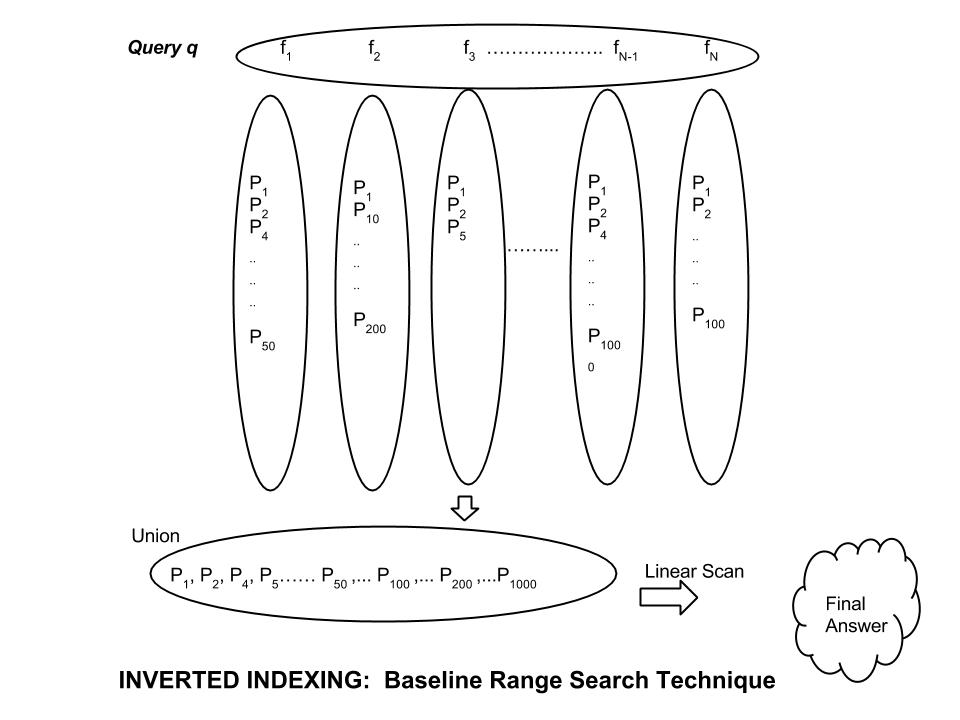
\includegraphics[width=1 \columnwidth]{img/image0c.jpg}
\caption{Inverted Indexing: Procedure Diagram}
\label{fig: invert}
\end{figure}




\section{Pruning Features}
\label{sec:prune1}
 We use a greedy technique to prune features i.e. prune out features whose points are guaranteed to lie outside distance threshold.
 
\begin{enumerate}
	\item We sort the features of the query q, $f_1,f_2,...f_{N_q}$ in descending order of popularity i.e. the feature present in most of the points is at the start.
	
	\item We prune this feature if the maximum similarity value is less than the minimum required similarity threshold.
	
	\item Consider feature $f_1$. Let's say we want to prune this feature. We are concerned with points having this feature but not having any of the other features of the query point. 
	
	\item Let us assume binary fingerprints for simplicity. The maximum similarity such a point can have with the query point is $\frac{1}{N_q - 1 + V_{1}}$ where $N_q$ is the number of features in query q and $V_{1}$ is the minimum number of features present among all points having the feature $f_1$
	
	\item Hence if  distance threshold is t and the following holds
	\[\frac{1}{N_q - 1 + V_{1}}  < 1-t\]
we can prune the feature $f_1$		
	
	\item We continue a greedy approach, where we consider the next feature $f_2$ and try to prune both the features $f_1$ and $f_2$ together.
	
	\item Hence if till the $i^{th}$ feature is considered, if j features have been pruned, we can prune the $i^{th}$ feature as well if the following holds
	\[\frac{j+1}{N_q - 1 + min(V_{i}, \rho)} < 1-t \] where $\rho$ is the minimum number of features present in any of the compounds of the features pruned till now.
	
\end{enumerate}

\section{Extension to non-binary fingerprints}	
\label{sec:prune2}
We can extend this to non binary fingerprints as well. In step 5 of the previous algorithm, while considering non-binary fingerprints we have to use the following inequality to determine if feature $f_1$ can be pruned.

\[\frac{min(j_1,W_1)}{S_q - W_1 -k_1 + l_1 + max (k_1, V_1)}  < 1-t\]

Here $j_1$ is the maximum feature value taken for the feature $f_1$, $W_1$ is the first feature value of query $q$, $S_q$ is the sum magnitude of the feature values of the query $q$, $k_1$ is the is the minimum feature value taken for the feature $f_1$, $l_1$ is the minimum sum of feature values for any point containing the feature $f_1$ and $t$ is the threshold similarity

Hence if till the $i^{th}$ feature is considered, if j features have been pruned, we can prune the $i^{th}$ feature as well if the following holds:
		

\[\frac{\sum\limits_{i \in J}min(j_i,W_i)}{S_q - \sum\limits_{i \in J}W_i -\sum\limits_{i \in J}k_i + max_{i \in J}l_i + \sum\limits_{i \in J}max (k_i, V_i)}  < 1-t\]
	
Here $J$ is the set of features already pruned,$j_i$ is the maximum feature value taken for the feature $f_i$, $W_i$ is the $i^th$ feature value of query $q$, $S_q$ is the sum magnitude of the feature values of the query $q$ as mentioned earlier, $k_i$ is the is the minimum feature value taken for the feature $f_i$ , $l_i$ is the minimum sum of feature values for any point containing the feature $f_i$ and $t$ is the threshold similarity




\section{Using the Minimum Similarity Bound}

Just like in the M-tree, similar to using the triangle inequality bounds, instead of using the maximum possible similarity, we used the minimum possible similarity and use it to include all points contained by a feature.

Hence for a feature $f_1$ of a binary fingerprint query $q$, we can include all points having feature $f_1$ in our result set if the following inequality holds
	\[\frac{1}{N_q - 1 + U_{1}}  > 1-t\]
Here $N_q$ is the number of features in query q and $U_{1}$ is the maximum number of features present among all points having the feature $f_1$. This holds true because the right hand side of the bound represents the least possible similarity between the query and any compound having feature $f_1$. If the left hand side is greater than the similarity threshold s ($s=1-t$), than we need not undergo the min-max similarity calculation for all the chemical fingerprints.

This is a very loose lower bound and hence we observed in our results that we were unable to exploit this bound for speeding up our process.
	


\section{Splitting Features}

Another technique we considered for the binary dataset is the splitting of the heavy hitting features into two sets so that we can prune atleast the bigger set. If the bound for pruning the feature fails, then we try to split the feature into two sets so that the minimum number of features for any point in one of the sets increases and then giving a chance of the set being pruned. For this we have to sort the points in the feature in ascending order of the number of features present in the point .This procedure is applied only for the heavy hitting features since they appear in a large number of points. If we were to apply this to other features, the time spent partitioning would exceed the probable time spent in comparing all points in the partition to the query. Hence we would like to apply this only to features which are present in more than a threshold number of points.\\

\begin{figure}[ht]	
\centering
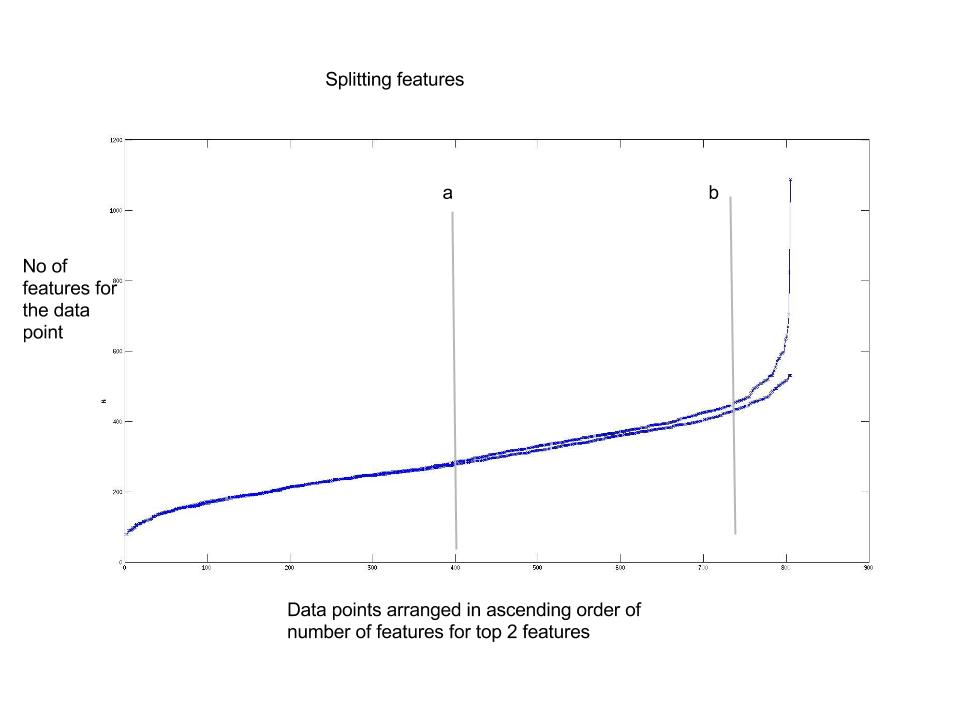
\includegraphics[width=1 \columnwidth]{img/feat_split.jpg}
\caption{Inverted Indexing: Splitting the heavy hitting features}
\label{fig:split}
\end{figure}

\autoref{fig:split} shows the number of features versus every point present for two heavy hitting features. It can be observed that the curve is almost linear, hence intuitively we wouldn't get a very large increase in the minimum number of features for the larger set of points.In \autoref{fig:split}, we can observe two lines \textit{a} and \textit{b}. If we were to split at \textit{a}(into approximately two equal sets) after sorting, our pruning bound would have a lower chance of getting  satisfied while if we were to cut at \textit{b}(at about 90\% to 10\%) we would have a better chance of pruning the set containing the top 10 percent of the points.